\chapter{传统的基于统计的命名实体识别方法综述}
本章从语言模型入手,介绍了当前常见的几种基于统计的命名实体识别方法,包括以马尔可夫模型为基础的隐马尔可夫模型、结合了最大熵模型的最大熵马尔可夫模型,将命名实体识别任务转化为文本分类问题的支持向量机方法,以及目前工业界最常用,并且具有很好效果的条件随机场方法。
最后,我们通过比较这几种方法的原理和在命名实体识别任务上的性能,分析了传统的基于统计的命名实体识别方法的局限性;
同时,针对二元语言模型、隐马尔可夫模型,探讨了它们对基于神经网络的方法存在的潜在改进思路;
最后,针对条件随机场模型,探讨了其与神经网络相结合的原理和意义。
\section{隐马尔可夫模型与最大熵马尔可夫模型}
\label{chap:HMM}
隐马尔可夫模型和结合了最大熵方法的最大熵马尔可夫模型在解决序列标注问题得到了被广泛应用,其中隐马尔可夫模型还在语音识别、统计机器翻译上有着重要的应用。
\subsection{预备知识}
在介绍上述两种模型之前,需要先对n元语言模型和一般的马尔可夫模型做简要的介绍。
语言模型是一种构建简单、直接的模型,是人们对语言这一抽象概念的一种相对简单的数学形式化。
语言模型实际上是针对特定语料集的统计特征建立的模型。
一般来说,对于给定的文本序列
\begin{equation}
    S = w_1 w_2 w_3 \dots w_n
\end{equation}
在语言模型下,该文本序列可判定为句子的概率$P(S)$即为模型的输出,其中$w_i, i\in \{1,2,\dots,n\}$称为文本序列的基本元素,基本元素可以是字,典型的如中文、日文等;也可以是词,如英文、法文等西方语言;也可以是其他人为规定的文本元素。
概率$P(S)$可由下式计算:
\begin{align}
    P(S) &= P(w_1)P(w_2 | w_1)P(w_3 | w_1 w_2)\cdots P(w_n | w_1 w_2 \cdots w_{n-1}) \label{eq:n-gram}\\
    &= \prod_{i=1}^{n}P(w_i | w_1 \cdots w_{i-1})
\end{align}

可以看出,产生第$i$个基本元素的概率依赖前面所有的基本元素,则随着句子长度的增加,需要估计的参数就会呈指数级增加。这种规模的参数很难从有限的训练样本中准确估计,其计算量所需要的时间成本也难以接受。

在式\ref{eq:n-gram}的基础上,若假设产生第$n$个基本元素的概率不再依赖前面的所有基本元素,而只依赖它之前的$n-1$个,则称该语言模型为n元语言模型(n-gram)。
当$n=1$时,即每个基本元素的出现是独立的,不依赖其前面的基本元素,则称该模型为一元语言模型(uni-gram);当$n=2$时,即每个基本元素的出现仅与它前面的一个元素相关,则称该模型为二元语言模型(bi-gram),且注意到一阶离散马尔可夫链的性质:
\begin{equation}
    P\{X_{n+1} = x|X_1 = x_1, X_2 = x_2, \dots, X_n = x_n\} = P\{X_{n+1} = x| X_n = x_n\}
\end{equation}
其中$X_1, X_2, \dots , X_n$是随机状态序列,$x_1, x_2, \dots, x_n$是过程中的状态,则可知随机状态序列中$X_{n+1}$关于之前所有序列元素的条件概率分布是只关于${X_n}$的函数,即在该随机状态序列中,某时刻状态只与其前一时刻的状态有关。
上述二元语言模型满足此性质,则二元语言模型是一个马尔可夫模型;当$n=3$时,第$n$个基本元素与其之前的两个元素相关,称为三元语言模型(tri-gram),显然三元语言模型不满足马尔可夫性,故它不能称为马尔可夫模型。
但一般来说,对于$n\geq 3$的语言模型来说,其状态空间可描述为多个二元状态的乘积,则此时可将多元语言模型转化为马尔可夫模型,$n$元语言模型依赖前面$n-1$个元素,称为$n-1$阶马尔可夫模型。

以二元语言模型为例,假定以词为文本序列的基本元素,我们可以将它依据训练语料进行文本序列概率预测的过程理解为两个步骤:首先,使用训练语料建立词-词的转移矩阵,即两个词相邻,则存在一次前词到后词的转移;随后,计算待预测序列中所有存在的2-gram的概率,即估计
\begin{equation}
    P(w_i|w_{i-1}) = \frac{c(w_{i-1}w_i)}{\sum_{w_i}c(w_{i-1}w_i)}
\end{equation}
其中$w_i$是词,$c(w_{i-1}w_i)$是2-gram序列$w_{i-1}w_i$在训练语料中的频数。
最后计算序列条件概率:
\begin{equation}
    P(S) = \prod_{i=1}^{l+1}P(w_i|w^{i-1}_{i-n+1})
\end{equation}
其中$w^j_i$表示词序列$w_i,\dots,w_j$,且约定元素$w_{-n+2}$到$w_0$为统一的序列起始元素\verb|<BOS>|,$w_{l+1}$为统一的序列结束元素\verb|<EOS>|。

对于n元语言模型,存在着两方面的问题。
我们以中文和2-gram为例进行讨论。
首先不论是以词为单位还是以字为单位统计2-gram,由于语料总是有限的,无论规模多么庞大的语料总不可能会覆盖每两个词的组合,即一定会有部分2-gram序列$w_p w_q$其经过统计计算得到的$P(w_p|w_q)=0$,于是所有以该2-gram为子序列的文本序列(句子)在该语言模型下的预测概率都将是0。
这显然不符合实际,因为一句话未曾在训练语料出现过,并不代表它不可能出现。
实际上,这种2-gram存在的数量还很多,导致词-词转移矩阵会非常稀疏,预测的结果也会受到严重影响。
这一问题称为数据平滑问题,解决这一问题基本思路是给予所有统计概率为0的2-gram以一个较小的非零概率,具体包括加一平滑、古德-图灵法等,限于篇幅,这里就不再详细讨论。

其次,进行这种模型的构建需要统计大量的词共现信息,谷歌进行的google books ngram项目中,中文的n-gram($n\in[1, 2, \dots, 5])$数量已经达到了百亿级别,如何有效存储、检索和计算如此规模的数据,也是其应用的一个问题\citep{宗成庆2013统计自然语言处理}。
\subsection{隐马尔可夫模型}
一般的马尔可夫模型,其状态和状态的转移都是可观测的。
如果可观测的结果并非是马尔可夫模型真正的状态序列,而是状态序列的经随机函数映射的结果,且状态及其转移过程都是不可见的,则这种模型称为“隐马尔可夫模型”。
我们可以通过下列方式描述一个隐马尔可夫模型:
\begin{equation}
    \mu =(S, K, \Matrix{A}, \Matrix{B}, \Matrix{\pi})
\end{equation}
其中,$S$为隐藏状态的集合,$K$为可能输出结果集合,$\Matrix{A}$、$\Matrix{B}$、$\Matrix{\pi}$分别是隐藏状态的转移概率矩阵、隐藏状态到输出结果的概率分布矩阵和隐藏状态的初始概率分布。一个典型的HMM模型结构可如图\ref{fig:HMM}所示。
\begin{figure}[H]
    \centering
    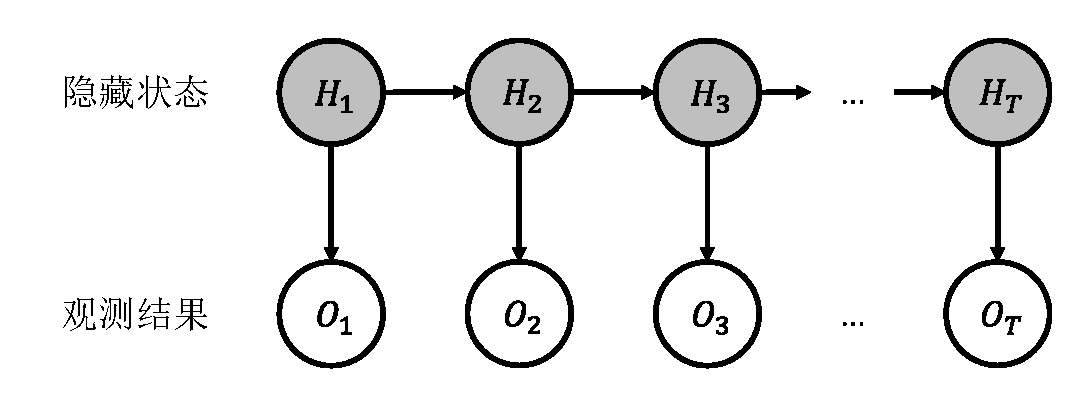
\includegraphics[width=0.8\textwidth]{HMM}
    \bicaption{HMM模型结构图}{HMM model structure}
    \label{fig:HMM}
\end{figure}
设$S=\{s_m|1\leq m \leq M\}$,即存在$M$种隐藏状态;$O=\{o_n|1\leq n\leq N\}$,即存在$N$种可观测到的输出结果,则$\Matrix{A}$中元素$a_{ij}$满足:
\begin{align}
    a_{ij} &= P(q_t = s_j|q_{t-1} = s_i)\qquad 1\leq i,j \leq M\\
    a_{ij} &\geq 0 \label{eq:norm-1}\\
    \sum^{N}_{j=1}a_{ij} &= 1 \label{eq:norm-2}
\end{align}
$a_{ij}$称为状态从$s_j$转移到$s_i$的归一化概率(满足式\ref{eq:norm-1}和\ref{eq:norm-2},下同)。

与其类似,$\Matrix{B}$中元素是隐藏状态$s_j$到时刻$t$的输出结果$O_t$的归一化概率分布,即发射概率:
\begin{equation}
    b_j\{k\} = P(O_t = o_k |q_t = s_j)\qquad 1\leq j \leq M; 1\leq k\leq N
\end{equation}

隐藏状态的初始概率分布$\Matrix{\pi_i}$同样为初始状态的归一化概率分布,定义为:
\begin{equation}
    \pi_i = P(q_1 = s_i)\qquad 1\leq i \leq N
\end{equation}

由上述定义可知,隐马尔可夫模型中隐藏状态序列由$\Matrix{\pi}$和$\Matrix{A}$决定,输出的结果,即观察序列由$\Matrix{B}$决定。

对于命名实体识别问题,我们可以将语料中可以观测到的字词理解为观察序列,其所对应的标签序列(是否是命名实体)为隐藏状态序列。
给定观察序列$O = O_1 O_2\dots O_T$和模型参数$\mu = (\Matrix{\pi},\Matrix{A},\Matrix{B})$,则该观察序列在该模型下的概率可用下式表示:
\begin{align}
    &\forall Q = q_1 q_2 \dots q_T:\nonumber\\
    &\qquad P(O|\mu) = \sum_Q \prod_{t=0}^{T-1}a_{q_t q_{t+1}}b_{q_{t+1}}(O_{t+1})
    \label{eq:HMM-conditional-probability}
\end{align}
特别地,当$t=0$时,$a_{q_0 q_1}b_{q_1}(O_1) = \pi_{q_1}b_{q_1}(O_1)$。

模型的训练过程为,给定观察序列$O$,即以字或词为序列元素的训练语料来调节模型参数$\mu = (\Matrix{\pi},\Matrix{A},\Matrix{B})$,使得序列在该模型参数下的概率最大:
\begin{equation}
    \mathop{\arg \max}_\mu P(O|\mu)
\end{equation}
模型参数可使用基于Baulm-Welch算法的期望最大化(expectation maximization, EM)算法进行训练。

模型的预测过程(即解码过程)为,给定模型$\mu = (\Matrix{A},\Matrix{B},\Matrix{\pi}$和一个观察序列$O$,求可能的状态序列$\hat{Q}$,使得
\begin{equation}
    \hat{Q} = \mathop{\arg \max}_Q P(Q|O,\mu)
\end{equation}
预测过程的序列选择结果,可以由Viterbi算法得出。

\subsection{最大熵马尔可夫模型}
为了能够利用包括大写、词尾、词性、格式和词所处的位置信息等额外特征,McCallum等人在2000年提出了最大熵马尔可夫模型(maximum-entropy Markov model, MEMM)。
它与HMM的区别在于HMM是生成式模型,对于给定的文本序列(即观察序列)$S$和它们对应的标签(即隐藏状态序列)$O$,它估计的是隐藏状态序列与观察序列的联合概率$P(S,O)$;
而MEMM是判别式模型,它估计的是条件概率$P(S|O)$。
具体来说,在训练过程中,HMM给定观察结果$o$,调节模型$\mu$的参数使得$P(o|\mu)$最大,并且由于隐藏状态是不可观测的,需要使用EM算法训练参数;
而MEMM则是给定观察结果$o$和当前的隐藏状态$s$,调节模型参数使得$P(s|o,\mu)$最大。
在解码(预测)过程中,HMM计算$S$使得$P(O|S,\mu)$最大,MEMM计算$S$使得$P(S|O,\mu)$最大。
MEMM模型基本结构如图\ref{fig:MEMM}所示。

\begin{figure}[H]
    \centering
    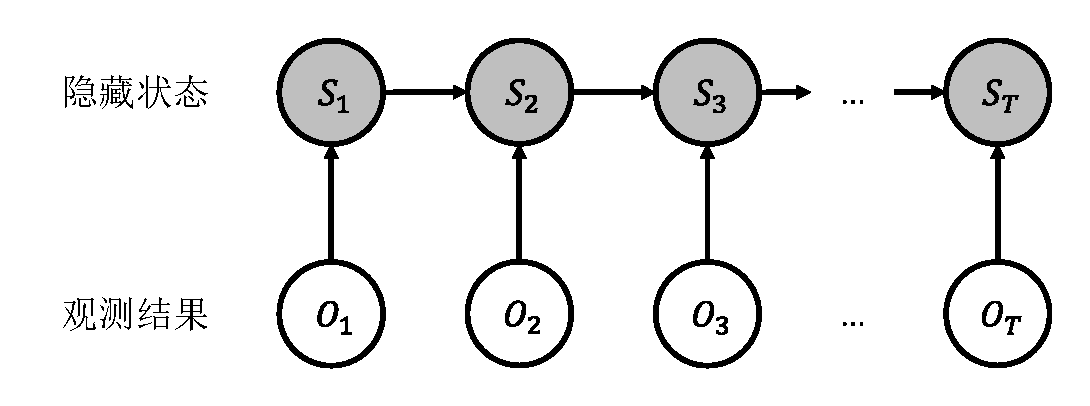
\includegraphics[width=0.8\textwidth]{MEMM}
    \bicaption{MEMM模型结构图}{MEMM model structure}
    \label{fig:MEMM}
\end{figure}

对于给定的观察序列$O_1 O_2\dots O_T$和状态序列$S_1 S_2\dots S_T$,MEMM的解码过程为:
\begin{equation}
    P(S_1\dots S_T|O_1\dots O_T) = \prod_{t=1}^{T}P(S_t|S_{t-1}, O_t)
    \label{eq:memm-decoding}
\end{equation}

由式\ref{eq:memm-decoding}可见,与式\ref{eq:HMM-conditional-probability}相比,MEMM将其中的两个条件概率分布替换为:
\begin{equation}
    P(s|s',o) = P_{s'}(s|o) = \frac{1}{Z(o,s')}exp(\sum_{a}\lambda_a f_a(o,s)) \label{eq:memm}
\end{equation}
其中$s'$为$S_{t-1}$的任意可能取值,$o$为当前时刻的观察结果$O_t$的取值,$Z(o,s')$为归一化因子,定义为:
\begin{equation}
    z(o, s') = \frac{P(s|s',o)}{\sum_{\tilde{s}}P(\tilde{s}|s',o)}
\end{equation}
$\lambda_a$为待估计的特征函数权重,$f_a(o,s)$为二值特征函数,用于获取额外的特征。定义为:
\begin{equation}
    f_a(o_t, s_t) = f_{\langle b,r\rangle}(o_t, s_t) = \left\{
        \begin{array}{ll}
        1, b(o_t) = True, s_t = r\\
        0, Other
        \end{array}
    \right.
\end{equation}
同时,MEMM还对训练过程中的Baulm-Welch算法和用于预测的Viterbi算法进行了修改,具体推导过程就不再赘述。

\section{支持向量机}
除了上述基于隐马尔可夫模型的命名实体识别方法之外,一些常用于分类问题的机器学习方法也能够应用于命名实体识别任务上。
本节将简要介绍支持向量机方法在命名实体识别中的应用。
支持向量机是针对二分类问题提出的一种分类方法。在该方法下,对训练数据集的描述为:
\begin{equation}
    D = {(\Vector{x_1}, y_1), (\Vector{x_2}, y_2), \dots, (\Vector{x_m}, y_m)}, \Vector{x_i} \in \Set{R}^N, y_i \in \{-1, +1\}
\end{equation}
其中$\Vector{x_i}$是第$i$个训练样本的特征向量,$y_i$是样本的标签,即正例或负例。
基于该样本集我们需要找到一个二值的决策函数来预测未在训练样本中出现过的$\Vector{x}$的标签$y$:
\begin{equation}
    f(\Vector{x}) = sign(g(\Vector{X}))
\end{equation}
即若$f(\Vector{x}) = +1$,则样本属于某类;若$f(\Vector{x}) = -1$,则样本不属于某类。

若样本集是线性可分的,则其中$g(x)$表示为:
\begin{align}
    g(\Vector{x}) &= \Vector{w}^{\mathrm{T}}\Vector{x} + b\\
    &= \sum_{i = 1}^m w_i\Vector{x_i}^{\mathrm{T}}\Vector{x} + b
\end{align}
若样本集是线性不可分的,则其中$g(x)$可进一步表示为更一般的形式:
\begin{align}
    g(\Vector{x}) &= \Vector{w}^{\mathrm{T}}\Vector{x} + b\\
    &= \sum_{i = 1}^m w_i K(\Vector{x}, \Vector{x_i}) + b
\end{align}
其中$K(\Vector{x}, \Vector{x_i})$为核函数,它的作用是将样本空间映射到一个线性可分的空间,从而将线性不可分的问题转化成线性可分的问题,再求解超平面实现分类,如图\ref{fig:SVM}\citep{alisneakysvm}所示。

\begin{figure}[H]
    \centering
    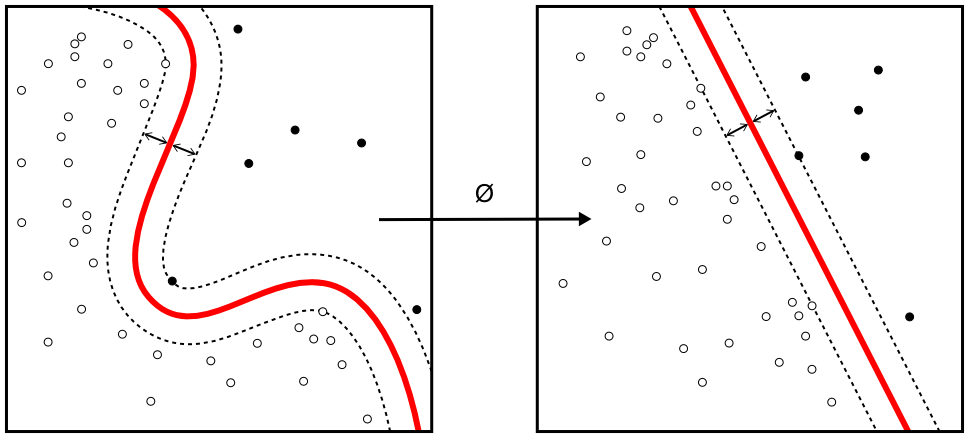
\includegraphics[width=0.8\textwidth]{SVM.png}
    \bicaption{SVM使用核函数将样本映射到高维空间}{SVM projects samples to a higher dimension space using kernel functions}
    \label{fig:SVM}
\end{figure}

可以看出,若核函数取$K(\Vector{x_i}, \Vector{x_j}) = \Vector{x_i}^{\mathrm{T}}\Vector{x_j}$则模型就是线性可分的形式,因此这个核函数也称为线性核。
除此之外,还有多项式核$K(\Vector{x_i}, \Vector{x_j}) = (\Vector{x_i}^{\mathrm{T}}\Vector{x_j})^d, d>1$,高斯核$K(\Vector{x_i}, \Vector{x_j}) = exp(-{\lVert\Vector{x_i} - \Vector{x_j}\rVert^2}/{2\sigma^2})$等,核函数的选择对分类的效果起着至关重要的作用,因此也是一个重要的研究方向。

\citet{isozaki2002efficient}使用了SVM进行命名实体识别。首先,训练样本中的每一个词都表示为包含15个特征的向量形式,这15个特征是指,以当前词为中心,前后各两个词共五个词各自的词性、词形(大小写)和词典位置(这部分类似one-hot向量)。
经拼接后得到一个39000多维的特征向量作为词的表示。
接着,使用多个独立的SVM分类器对这些向量进行分类。这一过程中可能出现多个分类器判定是该类别,或者没有分类器判定是该类别的情况,通常的做法是通过比较$g_c (\Vector{x})$的值,选取一个最大值来确定其类别$c$。
但为了避免不合理的序列出现,如标记为人名起始词后面应该是人名中间词或人名结束词,该方法同样使用了Viterbi算法来在可行的序列空间中获取出现概率最大的序列。由于SVM的输出并非概率值,文中使用\verb|Sigmoid|函数来将SVM的输出结果$g_c (\Vector{x})$映射到概率空间。
在日文数据集上,使用569994个特征向量训练的结果显示,该方法的F值最高达到了88.31\%,优于最大熵模型和基于规则的决策树模型。

尽管在获得了足够的训练数据后,SVM能够给出相对可靠的命名实体识别结果,但其问题在于,首先特征向量非常稀疏,造成来大量的空间浪费,这种情况随着训练数据的增多会更加严重;其次由于特征向量维数巨大,其运算资源消耗并不小,因此造成SVM的训练速度较慢。

\section{条件随机场}
条件随机场(CRFs)与MEMM同属判别式模型,且都能够定义额外特征,在自然语言处理中得到了广泛的应用。

设随机变量$X$为表示观察序列的随机变量,$Y$为表示与观察序列对应的标签序列的随机变量。则条件随机场建模的目标是给定序列$X$的情况下,序列$Y$的条件概率$P(Y|X)$。条件随机场可以通过满足一定马尔可夫假设的无向图模型来描述。

设图$G=(V,E)$,标记序列$Y = (Y_v)_{v\in V}$,则序列元素$Y_v$与图中节点一一对应。若给定序列$X$,随机变量$Y_v$在图中满足马尔可夫性:
\begin{equation}
    p(Y_v|X, Y_w, w\neq v) = p(Y_v|X,Y_w,w\sim v)
    \label{eq:Markov-in-CRF}
\end{equation}
其中$w\sim v$表示$w$和$v$为图中的邻接结点。则$(X, Y)$构成一个条件随机场。针对命名实体识别这类序列标注问题,一般可以令$G$为链式结构,即构成线性链式条件随机场。一个典型线性链式条件随机场的无向图表示可如图\ref{fig:CRF}表示。

\begin{figure}[H]
    \centering
    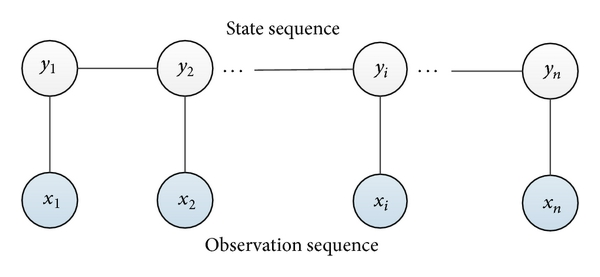
\includegraphics[width=0.8\textwidth]{CRF}
    \bicaption{CRF的链式无向图模型}{Chained undirected graph of CRF}
    \label{fig:CRF}
\end{figure}

条件随机场可以视为是满足一定条件的的马尔可夫网络。在马尔可夫网络中,结点序列的联合概率分布可以表示为图中关于序列结点的所有完全子图(团)的势能函数的乘积。设图中所有团的所有团的集合为$C = \{c|c$是图$G$上的团$\}$,于是有:
\begin{equation}
    P(Y) = \frac{1}{Z}\prod_{c}\psi_x(Y_c)
\end{equation}
其中$Z$为归一化参数,使结果可以视作概率:
\begin{equation}
    Z = \sum_Y\prod_c \psi_c(Y_c)
\end{equation}
式中乘积的因子即势能函数。

在线性链式条件随机场中,每个${Y_i, X_i}$即一个团,且由式\ref{eq:Markov-in-CRF}知:
\begin{equation}
    P(Y_i|X, Y_j, j\neq i) = P(Y_i|X, Y_{i-1})
\end{equation}
则可得到公式:
\begin{equation}
    P(Y|X) = \frac{1}{Z}\prod_i\psi_i(Y_i|X)
\end{equation}
而给定观察序列$\Vector{X}$时,某特定标记序列$\Vector{Y}$的概率可定义为:
\begin{equation}
    exp(\sum_j\lambda_j t_j(y_{i-1}, y_i, X, i) + \sum_k \mu_k s_k(y_i, X, i))
\end{equation}
则有:
\begin{equation}
    P(Y|X) = \frac{1}{Z}exp(\sum_j\sum_{i=1}^{n-1}\lambda_j t_j(y_{i-1}, y_i, x, i) + \sum_k\sum_{i=1}^{n}\mu_k s_k(y_i, x, i))
\end{equation}
其中,$t(y_{i-1}, y_i, X, i)$是标签序列中相邻位置标签的转移特征函数,表示给定观察序列$X$时,相邻标签的转移概率;
$s_k(y_i, X, i)$是标签序列中位置$i$的状态特征函数,表示给定的观察序列$X$对该位置标签的影响;
$\lambda_j$和$\mu_k$分别是两种特征函数的权重,为模型需要训练的参数。

状态特征函数通常定义为一个$(0,1)$二值函数:
\begin{equation}
    s_(X, i) = \left\{
        \begin{aligned}
            1, &\qquad if~X_i = "Me"\\
            0, &\qquad Other
        \end{aligned}
    \right.
\end{equation}

类似地,状态函数则联合状态特征和前后标签约束输出特征结果:
\begin{equation}
    t_(y_{i-1}, y_i, X, i) = \left\{
        \begin{aligned}
            1, &\qquad if~d X_i = "Me" ~ d and ~ d y_{i-1} = L_1, y_i = L_2\\
            0, &\qquad Other
        \end{aligned}
    \right.
\end{equation}

CRF的训练过程一般基于对数似然函数最大化进行,解码过程与HMM类似,利用Viterbi算法在可能的隐藏状态序列空间中寻找概率最大的隐藏状态序列。

\section{基于统计方法的比较和分析}
n元语言模型直接针对语料库中词前缀序列与词的转移概率建模,依靠对大规模语料库的统计获得模型的参数。虽然统计得到的转移概率能够在一定程度上体现词之间的共现特征,但作为基于统计的语言模型,较难考虑到语句中的语法和语义特征;又因为其统计的上文窗口有限,既难以获取距离较远的上文依赖特征,又忽略了重要的下文特征。并且,直接对语料建模统计出的语言模型,是严重依赖语料本身的质量和特性的,对于不同领域的语料,统计得到的n-gram模型可能有较大差异。总的来说,独立使用n语言模型无论在效果、适应性还是在模型的计算、存储上都存在一定的局限性。

\citet{张华平2004基于角色标注的中国人名自动识别研究}实现的ICTCLAS采用三层层叠隐马尔可夫模型进行命名实体识别。
该方法针对人名、地名和组织机构名分别建立了三层隐马尔可夫模型进行三种命名实体的识别,并分别建立了人名、地名和组织机构名的角色表,即每层隐马尔可夫模型的隐藏状态集合。
该方法首先对原始语料进行切分,得到以词性为标签集的切分语料库;
接着在切分语料库的基础上,以人名角色表为标签集标注语料库,得到人名角色词典,并训练人名角色的转移概率,即识别人名的隐马尔可夫模型参数;
随后根据人名词典,得到识别人名之后的语料库,再以地名角色表为标签集标注语料库,得到地名角色词典,并训练识别地名的隐马尔可夫模型参数;
最后在识别了人名、地名的语料库上以组织机构名为标签集标注语料库,得到组织机构名词典,并训练最后一层隐马尔可夫模型参数。
基于层叠隐马尔可夫模型角色标注的命名实体识别方法,在《人民日报》语料集上的开放测试中,人名、地名和组织机构名识别的F1值分别达到了84.25\%、85.64\%、73.78\%。

与n元语言模型的情况类似,HMM也存在自身的局限性。
HMM模型建立在三个基本假设上,即
\begin{enumerate}[leftmargin=*]
    \item[(1)] 马尔可夫假设(Markov assumption):后一时刻隐藏的状态仅与当前隐藏时刻的状态相关
    \item[(2)] 稳定性假设(Stationarity assummption):状态转移概率与转移发生的时刻无关
    \item[(3)] 输出独立假设(Output independence assumption):给定当前时刻的状态时,当前时刻的观测输出与之前的观测输出都无关
\end{enumerate}
基于上述三个假设,HMM的局限性体现在三个方面。
首先,马尔可夫性要求,模型某一时刻的隐藏状态只与其前一时刻的状态相关,这一基本假设限制了模型既不能考虑序列后文的信息,也不能考虑距离较远的前文信息;
其次,上述基本假设下的模型也很难完整地抽象自然语言的各类统计特征,不论是词汇还是句法,都较该假设下的模型复杂得多;因此需要信息更为丰富、可以整合多种不同特征的词表示(word representations)。
最后,单纯依靠对语料建模得到的统计概率进行命名实体识别,是带有较强的领域特征的,模型的可移植性受到了较大的影响。
因此,尽管基于HMM的命名实体识别方法已经得到了广泛的应用,但其很大程度上还是依赖词典来保证识别的效果。

MEMM在HMM的基础上结合了最大熵模型的优点,对序列中的每个状态建立指数模型,以观察序列的特征作为输入,输出下一时刻状态的分布。这使得模型能够利用更多的额外特征,训练过程中也不需要遍历观察序列所有可能的值,能够从相对有限的信息中进行序列预测。
且由于MEMM对式\ref{eq:memm}中的每个条件概率可以由通过训练获得的收敛的特征函数权重$\lambda$和正则化因子$Z$直接求得,其求解过程相对独立,参数训练也较快。

但包括MEMM在内的非生成式条件马尔可夫模型,大多存在小概率的标记偏置(label bias)的问题。
考虑一个观察结果集$O$、状态集$S$、观察序列$X = x_1x_2x_3$和其对应的状态序列$Y = y_1y_2y_3$,若训练得到$y_1$可能的状态集合为$\{s_1, s_2\}$,而$y_2$可能的状态只有$s_3$,这种情况下意味着在给定观测结果$x_2$和前一时刻任意取值的状态$y_1$时,条件概率$P(y_2 = s_3|x_2, y_1) = 1$,因此有:
\begin{equation}
    P(y_2 = s_3|x_2, y_1 = s_1) = P(y_2 = s_3|x_2, y_1 = s_2) = 1
\end{equation}
在训练语料中,不妨设$P(y_1 = s_1|x_1) < P(y_1 = s_2|x_1)$,则此时序列中标记路径的选择就取决于$P(y_1 = s_1|x_1)$和$P(y_1 = s_2|x_1)$了。
此时不论转移概率$P(y_2 = s_3|y_1 = s_1)$是否比$P(y_2 = s_3|y_1 = s_2)$大,模型都将选择状态路径$s_2s_3\dots$而不考虑实际的观察序列。这就是一个极端情况:若当前状态结点的后继结点只有一个状态,模型将倾向无视观测序列,而以前一时刻状态和下一时刻之间的条件概率作为路径选择依据。

并且,与MEMM类似的条件概率模型还会将序列中对某一时刻状态的决策与之后时刻状态的决策独立对待。这就会出现“前言不搭后语”的情况,模型得出的标记序列可能并不符合真正的语言习惯,或者并不满足作为连续的上下文内部应该存在的依赖。

CRF模型在马尔可夫模型的基础上,既解决了HMM独立性假设的问题,也解决了MEMM的标记偏置问题,使得其对上下文的特征信息的利用更高效,模型的适用性更强。
MEMM之所以会产生标记偏置问题,是因为它对每个状态序列的指数模型做了局部归一。
条件随机场基于无向概率图模型,对整个序列标注结果做全局归一化,避免了标记偏置问题。并且由于模型并未对作为观测序列输入的特征之间做任何独立性假设,因此特征的制定更为灵活,不需要考虑它们之间存在的相关依赖。

值得一提的是,CRF在命名实体识别任务上可以作为传统机器学习方法的典型代表,在中文命名实体识别任务中取得了令人瞩目的效果。
但由于CRF较为依赖对待识别实体的特征选择,因此制定高效、准确的特征模板函数对CRF的性能影响较大,这对进行命名实体识别的研究人员对文本数据和任务场景的理解提出了更高的要求。

\section{本章小结}
本章介绍了隐马尔可夫模型、最大熵马尔可夫模型、支持向量机和条件随机场模型的相关背景知识和基本原理,并考察了每个方法在命名实体识别中的实际应用,针对各个方法的实现原理,分析了部分方法在效率和性能上的缺点和不足,讨论了各个方法在进行命名实体识别时的局限性。

